\documentclass[twocolumn,a4paper]{IEEEtranfr}
%\documentclass
% verbatim : pour afficher le contenu d'un fichier 
%
\usepackage{verbatim}
% gère les graphiques .jpg, .png ,\dots.
\usepackage[dvips]{graphicx}
%
% Pour la gestion de la couleur 
%
\usepackage{color}

%
% Formule chimique
%
\usepackage{chemfig}
%
% + de maths avec AMS
%

\usepackage{amsmath}
\usepackage{amssymb}
%
% Pour afficher des algorithmes
%
\usepackage{algorithm}
\usepackage{algorithmic}
\usepackage{listings}
%
% pour l'hypertexte
%
\usepackage{url}
\usepackage{hyperref}
% français
\usepackage[french]{babel}
% accents
%
% ucs 
% utf8x 
% 
\usepackage{ucs}
\usepackage[utf8x]{inputenc}
%\usepackage[T1]{fontenc}
\usepackage{subfigure}
\usepackage{framed}

\makeatother
% Placer vos figures et images dans les répertoires suivants
% Ne jamais mettre les noms de 
%
% Attention le / final est important 
\graphicspath{{./images/}{./figures/}{../presentation/images/}}

% alias
%
% A consommer sans modération
%
%

\newcommand{\blst}{\begin{lstlisting}}
\newcommand{\elst}{\end{lstlisting}}
\newcommand{\beqan}{\begin{eqnarray*}}
\newcommand{\eeqan}{\end{eqnarray*}}
\newcommand{\beqa}{\begin{eqnarray}}
\newcommand{\eeqa}{\end{eqnarray}}
\newcommand{\bear}{\begin{eqnarray}}
\newcommand{\ear}{\end{eqnarray}}
\newcommand{\bears}{\begin{eqnarray*}}
\newcommand{\ears}{\end{eqnarray*}}
\newcommand{\beq}{\begin{equation}}
\newcommand{\eeq}{\end{equation}}
\newcommand{\rref}[1]{(\ref{#1})}
\newcommand{\eref}[1]{\rref{#1}}
\newcommand{\gd}{\stackrel{.}{\geq}}
\newcommand{\ld}{\stackrel{.}{\leq}}
%%\newcommand{\eqref}[1]{(\ref{#1})}
\renewcommand{\r}{\right}
\renewcommand{\l}{\left}
\newcommand{\lbr}{\left \{ }
\newcommand{\rbr}{\right \} }
\newcommand{\Lbr}{\left [}
\newcommand{\Rbr}{\right ]}
\newcommand{\lp}{\left (}
\newcommand{\rp}{\right )}
%\newcommand{\mylabel}[1]{\label{#1}  \mbox{~~ \tiny \bf [ #1 ] } }
\newcommand{\mylabel}{\label}

%% Notations d'ensembles
\newcommand{\X}{{\cal X}}
\newcommand{\Y}{{\cal Y}}
%\newcommand{\C}{{\cal C}}
\newcommand{\D}{{\cal D}}
\renewcommand{\S}{{\cal S}}
\newcommand{\T}{{\cal T}}
\newcommand{\R}{{\cal R}}
\renewcommand{\H}{{\cal H}}
\newcommand{\V}{{\cal V}}
\renewcommand{\P}{{\cal P}}

%% variables
\newcommand{\eps}{\epsilon}
\newcommand{\real}{{\mathcal {R}}}
\newcommand{\complex}{{\mathcal {C}}}

%% scalaires
\newcommand{\err}{\mathcal{E}}
\newcommand{\dmin}{D_{\min}}
\newcommand{\dl}{D_\ell}
\newcommand{\tw}{\tilde{w}}
\newcommand{\tx}{\tilde{x}}
\newcommand{\ty}{\tilde{y}}
\newcommand{\ha}{h^a}
\newcommand{\dftd}{\tilde{d}}
\newcommand{\dftw}{\tilde{w}}
\newcommand{\dfty}{\tilde{y}}
\newcommand{\dfth}{\tilde{h}}
\newcommand{\Lagrange}{{\mathcal L}}
\newcommand{\Ntones}{N_c}
\newcommand{\hk}{h^{(k)}}
\newcommand{\rh}{{\tt h}}
%%\renewcommand{\ell}{l}

%% vecteurs
\newcommand{\vR}{{\bf R}}
\newcommand{\vmu}{\mbox{\boldmath$\mu$}}
\newcommand{\vbreve}[1]{\v{#1}}
%\renewcommand{\v}[1]{{\bf #1}}
\newcommand{\xmmse}{\hat{\vx}_{{\rm mmse}}}
\newcommand{\va}{{\bf a}}
\newcommand{\vone}{{\bf 1}}
\newcommand{\vb}{{\bf b}}
\newcommand{\vm}{{\bf m}}
\newcommand{\vw}{{\bf w}}
\newcommand{\vwul}{{{\bf w}_{\rm ul}}}
\newcommand{\wul}{{{w}_{\rm ul}}}
\newcommand{\vwdl}{{{\bf w}_{\rm dl}}}
\newcommand{\wdl}{{{w}_{\rm dl}}}
\newcommand{\vs}{{\bf s}}
\newcommand{\vy}{{\bf y}}
\newcommand{\vyul}{{{\bf y}_{\rm ul}}}
\newcommand{\yul}{{{y}_{\rm ul}}}
\newcommand{\pul}{{{P}_{\rm ul}}}
\newcommand{\vydl}{{{\bf y}_{\rm dl}}}
\newcommand{\ydl}{{{y}_{\rm dl}}}
\newcommand{\pdl}{{{P}_{\rm dl}}}
\newcommand{\vz}{{\bf z}}
\newcommand{\vr}{{\bf r}}
\newcommand{\vc}{{\bf c}}
\newcommand{\vh}{{\bf h}}
\newcommand{\vg}{{\bf g}}
\newcommand{\vx}{{\bf x}}
\newcommand{\vxul}{{\bf x}_{\rm ul}}
\newcommand{\xul}{{x}_{\rm ul}}
\newcommand{\vxdl}{{\bf x}_{\rm dl}}
\newcommand{\xdl}{{x}_{\rm dl}}
\newcommand{\vd}{{\bf d}}
\newcommand{\ve}{{\bf e}}
\newcommand{\vv}{{\bf v}}
\newcommand{\vt}{{\bf t}}
\newcommand{\vu}{{\bf u}}
\newcommand{\vP}{{\bf P}}
\newcommand{\vq}{{\bf q}}
\newcommand{\vp}{{\bf p}}
%\newcommand{\vg}{{\bf g}}
\newcommand{\vxN}{{\bf x}^{\bf N}}
\newcommand{\vyN}{{\bf y}^{\bf N}}
\newcommand{\tvw}{{\bf \tilde{w}}}
\newcommand{\tvx}{{\bf \tilde{x}}}
\newcommand{\tvy}{{\bf \tilde{y}}}
\newcommand{\tty}{y'}
\newcommand{\vxa}{{\bf x}^{\bf a}}
\newcommand{\vya}{{\bf y}^{\bf a}}
\newcommand{\vwa}{{\bf w}^{\bf a}}
\newcommand{\var}{{\bf e}_{\bf r}}
\newcommand{\vat}{{\bf e}_{\bf t}}
\newcommand{\vD}{{\bf D}}
\newcommand{\vY}{{\bf Y}}
\newcommand{\vW}{{\bf W}}
\newcommand{\vdftd}{{\bf \tilde{d}}}
\newcommand{\vdftw}{{\bf \tilde{w}}}
\newcommand{\vdfty}{{\bf \tilde{y}}}
\newcommand{\vdfth}{{\bf\tilde{h}}}
\newcommand{\dftmH}{{\bf \tilde{H}}}
\newcommand{\vdftx}{{\bf \tilde{x}}}
\newcommand{\vdfta}{{\bf \tilde{a}}}
\newcommand{\vxA}{{\bf x}^{\bf A}}
\newcommand{\vxB}{{\bf x}^{\bf B}}
\newcommand{\vxAl}{{\bf x}^{\bf A}_{\bf \ell}}
\newcommand{\vxBl}{{\bf x}^{\bf B}_{\bf \ell}}
\newcommand{\rl}{r^{(\ell)}}
\newcommand{\wl}{w^{(\ell)}}
%% matrices
\newcommand{\mQ}{{\bf Q}}
\newcommand{\mU}{{\bf U}}
\newcommand{\mV}{{\bf V}}
\newcommand{\mPsi}{{\bf \Psi}}
\newcommand{\mUt}{{\bf U}_t}
\newcommand{\mUr}{{\bf U}_r}
\newcommand{\mX}{{\bf X}}
\newcommand{\mLambda}{\mathbf{\Lambda}}
\newcommand{\mF}{{\bf F}}
\newcommand{\mK}{{\bf K}}
\newcommand{\mG}{{\bf G}}
\newcommand{\mA}{{\bf A}}
\newcommand{\mB}{{\bf B}}
\newcommand{\mC}{{\bf C}}
\newcommand{\mD}{{\bf D}}
\newcommand{\mR}{{\bf R}}
\newcommand{\mH}{{\bf H}}
\newcommand{\mHa}{{\bf H^a}}
\newcommand{\mI}{{\bf I}}
\newcommand{\mk}{{\bf K}}
\newcommand{\mv}{{\bf V}}
\newcommand{\mO}{{\bf O}} %% orthogonal 
\newcommand{\mJ}{{\bf J}} %% pseudo covariance
\newcommand{\rH}{{\tt H}}
%%\newcommand{\dftmH}{\tilde{\mH}}
\newcommand{\sm}[1]{\sum_{#1=-\infty}^{+\infty}}
\newcommand{\smr}[3]{\sum_{#1=#2}^{#3}}
\newcommand{\smu}[1]{\sum_{#1=1}^{+\infty}}
\newcommand{\smz}[1]{\sum_{#1=1}^{+\infty}}
\newcommand{\ejm}[1]{e^{-j\omega #1}}
\newcommand{\ejp}[1]{e^{j\omega #1}}
\newcommand{\usdp}{\frac{1}{2\pi}}
\newcommand{\edjm}[1]{e^{-j 2\pi f #1}}
\newcommand{\edjp}[1]{e^{j 2\pi f #1}}
%% math notation
\newcommand{\sinc}{{\rm sinc}}
\newcommand{\CN}{\mathcal{CN}}
\newcommand{\N}{\mathcal{N}}
\newcommand{\indistrib}{\stackrel{\mathcal{D}}{\rightarrow}} 
\newcommand{\inprob}{\stackrel{\mathcal{P}}{\rightarrow}}   
\newcommand{\mc}[1]{\mathcal{#1}}

%
%
%  Début du document 
%
%
\begin{document}

\title{Etude et mise en place d'Edge Node sur la base d'OpenEdgeComputing}
\author{HOANG Tuan Dung, KAF Merwan, LE CORRE Pierre} 

% place le titre 
\maketitle

\begin{abstract}
Avec l’arrivée massive des objets connectés, la bande passante du réseau internet risque d'être saturé par la trop grande demande de ressources faites aux serveurs situés dans le Cloud. Afin de palier à ce problème, Orange Labs a proposé l’étude d’une solution existante : OpenEdgeComputing. Cette solution consiste à se servir de la puissance de calculs de machines situés en périphérie du réseau (mini datacenter, livebox, ...) afin de permettre aux objets connectés d'accéder à de la puissance de calculs sans remonter jusqu'au serveurs situés dans le cloud. Dans un second temps, l'implémentation d'une nouvelle solution a été mis en oeuvre afin de palier aux problèmes de OpenEdgeComputing.

\end{abstract} 

\begin{keywords}
Cloudlet, Edge Node, Open Edge Computing, Open Stack, Cloud, Virtualisation, Zeroconf
\end{keywords}

%\markboth{This is for left pages}{and this is for right pages}


\section{Introduction}

Le projet confié par la société Orange s’inscrit dans l’anticipation de la multiplication future des objets connectés à internet. Ces derniers utilisent la puissance de calculs de serveurs distants très haut dans le réseau - que l’on appelle plus communément Cloud computing - afin d’effectuer divers traitement. Cependant, Orange estime que leurs nombres augmentera de façon tellement importante d’ici 5 à 10 ans que ces objets engorgeront le réseau ce qui altérera l’expérience des utilisateurs. Afin de palier à ce problème futur, Orange réfléchis à divers manières d’éviter aux objets connectés d’effectuer leurs traitements très haut dans le réseau. (cf. figure \ref{fig:cloud})


\begin{figure}[htpb]
  \begin{center}
    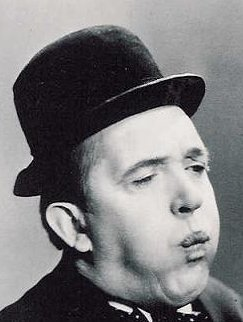
\includegraphics[width=0.7\columnwidth] {../images/SLaurel.jpg}
  \end{center}
  \caption{Schéma du cloud actuel}
  \label{fig:cloud}
\end{figure}

Le concept d’ Edge Computing permet de fournir de la puissance de calculs beaucoup plus bas dans le réseau et au plus proche des utilisateurs. L'intérêt est donc double, à la fois désengorger le réseau mais aussi diminuer la latence.
Dans ce projet le but est d’évaluer une solution open source : OpenEdgeComputing et de la mettre en oeuvre en proposant des outils spécifiques au besoin d’Orange.

\section{Contexte technique}

Dans le cadre de ce sujet, il peut-être utile de définir ou de rappeler certaines notions indispensables à la compréhension du projet : 
\begin{itemize}
\item Cloud computing : 
Ici la notion principale du cloud computing la plus pertinente pour ce projet est l’IAAS, traduction de “Infrastructure As A Service”, elle consiste à vendre des serveurs à une entreprise tiers, ainsi, celle-ci n’a plus à s’occuper du matériel sur lequel ses logiciels fonctionnent et peut, à tout moment, décider d’augmenter sa capacité de traitement, ou au contraire, la diminuer 
\item Edge computing
\begin{itemize}
\item Cloudlet : 
Une Cloudlet peut être considéré comme une sorte de mini-datacenter situé en périphérie du réseau internet, ici la périphérie d’internet est définie comme une zone géographique plus proche des utilisateurs. Un exemple est l’installation potentielle d’une Cloudlet dans le même espace que les antennes 4G (ou bientôt 5G)
\item OpenEdgeComputing : 
TODOTODTODOTODO
\end{itemize}
\item OpenStack : 
OpenStack est un ensemble de logiciels permettant de déployer un service de cloud-computing, que l’on nomme aussi IAAS (Infrastructure As A Service)
\end{itemize}

\section{Méthode} 

Trois phases distinctes définissent ce projet: 

\begin{itemize}
\item Recherche sur edge computing et plus spécifiquement sur le projet open source OpenEdgeComputing
\item Mise en place du projet OpenEdgeComputing
\item Mise en place d'une nouvelle solution
\end{itemize}

\subsection{Recherche sur OpenEdgeComputing}

La première partie du projet consistait en l’étude des différents projets EdgeComputing, et plus précisément celui de OpenEdgeComputing. Nous avons étudié l’architecture général des différents projets EdgeComputing (cf. figure représentant l’architecture).

En ce moment, il existe plusieurs notions dans le monde d’Edge Computing : Fog Computing, Mobile Edge Computing, Cloudlet, Micro datacenter. Ces notions sont prises en charge par des recherches menées par différentes organismes de recherche et d’entreprises. Cela explique pourquoi les notions Fog Computing, Mobile Edge Computing, Cloudlet, Micro datacenter sont à la fois ressemblantes et complémentaires.

\subsection{Mise en place de OpenEdgeComputing}

Le projet qui se base en grande partie sur le projet OpenStack qui permet de gérer un ensemble de serveur afin de constituer un cloud utilisable et manageable a été mis en place après l’installation d’Openstack sur un serveur.
En effet, le projet OpenEdgeComputing est en quelque sorte une surcouche d’Openstack simplifiant son utilisation avec des cloudlets en apportant quelques nouvelles fonctionnalitées : 

\begin{itemize}
\item La synthèse de machines virtuelles (VM Synthesis)
\item Une gestion de la continuité de certaines machines virtuelles (VM handoff)
\item Cartographie des Cloudlets pour sélectionner le plus proche (Discovery)
\end{itemize}


\begin{figure}[htpb]
  \begin{center}
    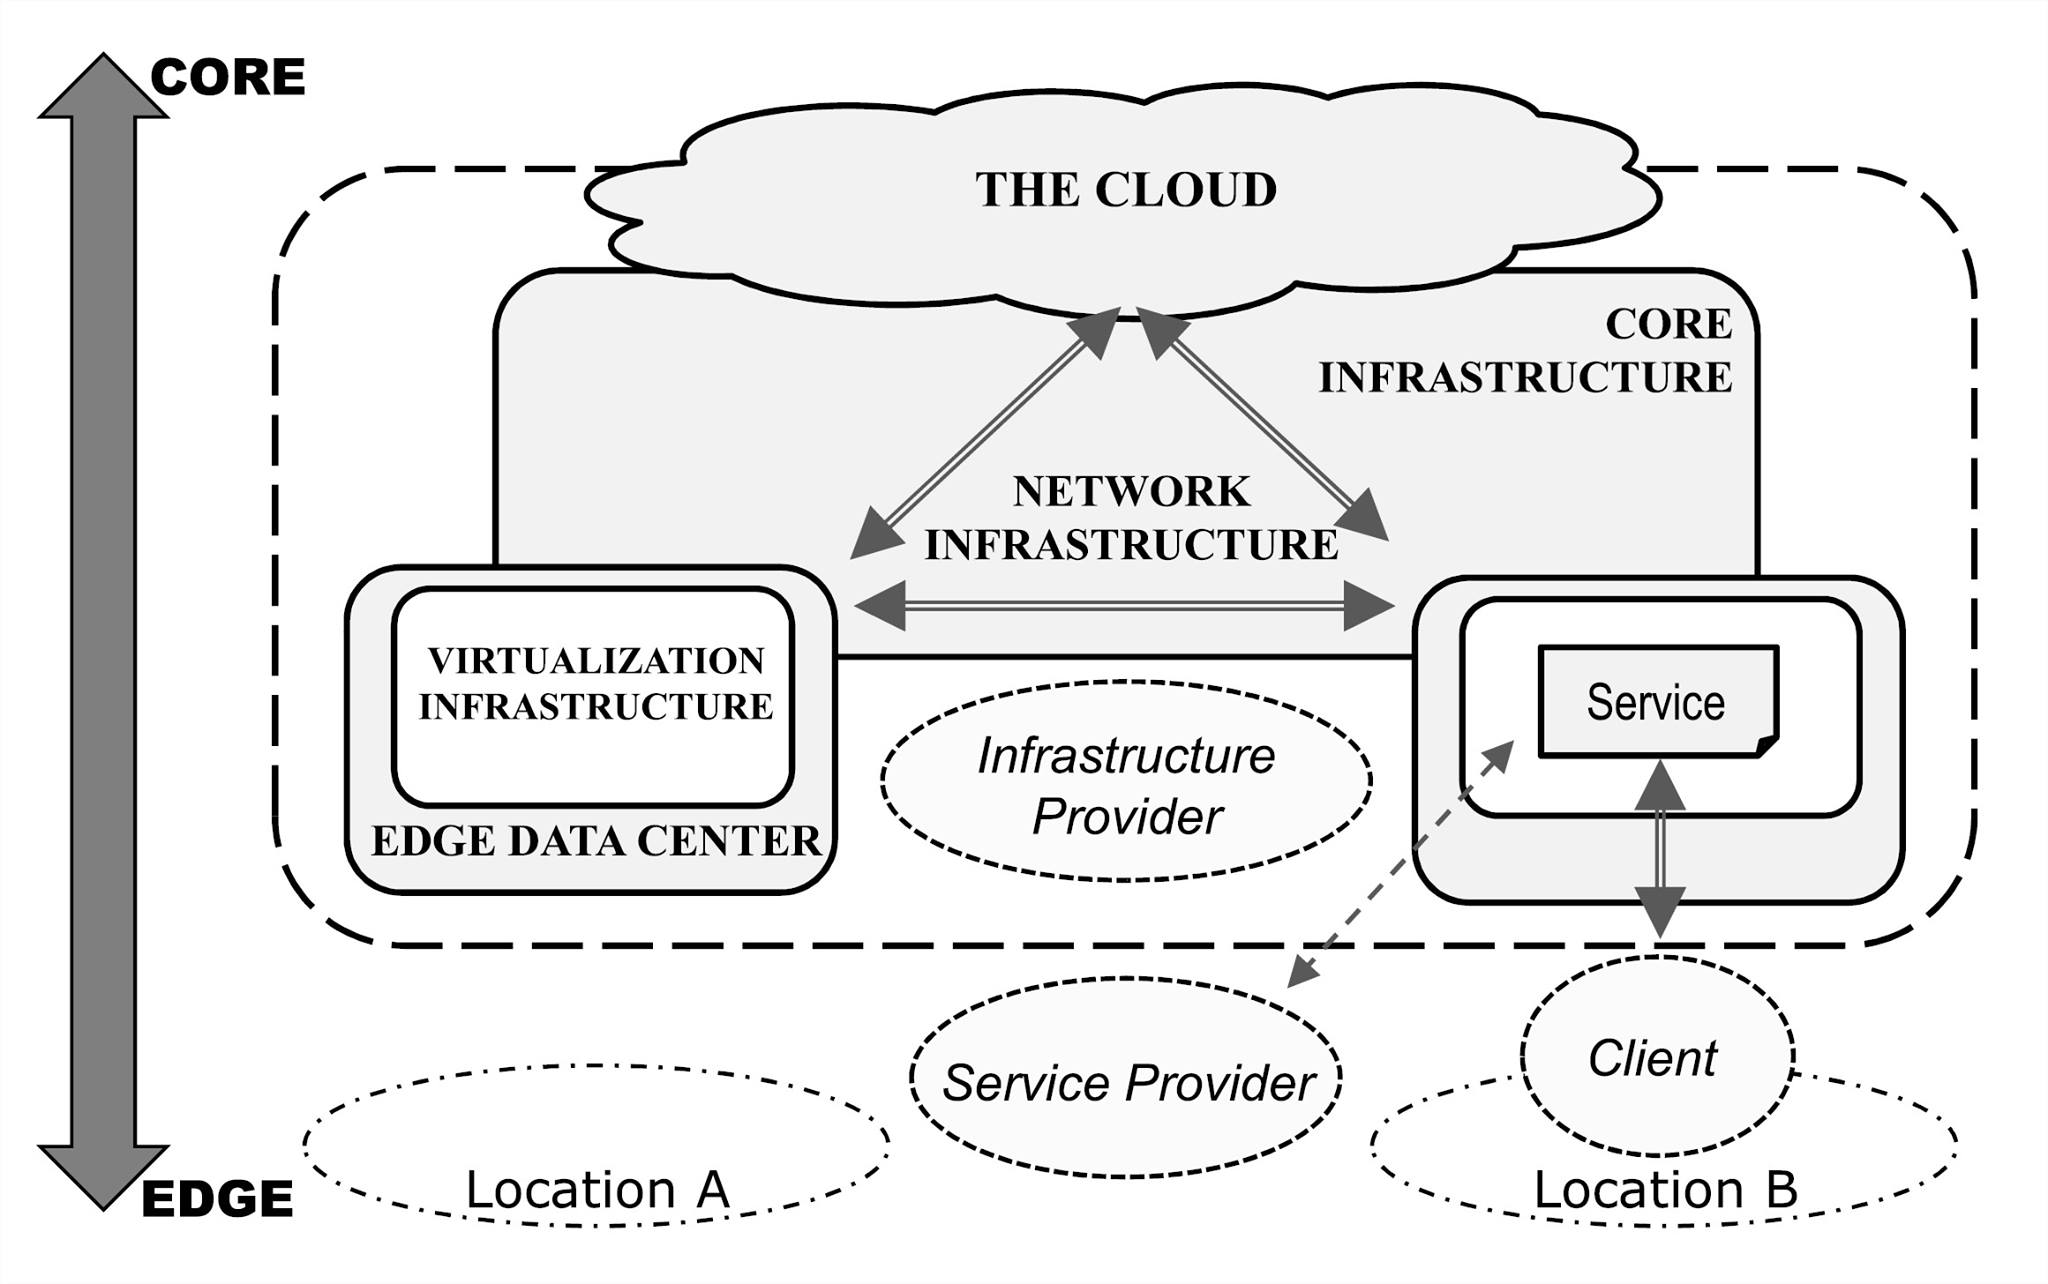
\includegraphics[width=0.8\columnwidth] {../images/open_edge.jpg}
  \end{center}
  \caption{Image OpenEdge  }
  \label{fig:openedge}
\end{figure}

La première partie consiste à installer Openstack Kilo, ensuite le projet OpenEdgeComputing possède plusieurs parties qui sont liées aux différentes fonctionnalitées ajoutées. La première à installer est la synthèse de machines virtuelle, elle consiste en l’installation d’une version modifiée de qemu ainsi que d’outils permettant la gestion de la synthèse de machines virtuelles.
La deuxième partie consiste en une modification de l’interface d’openstack, qui inclut désormais la gestion des cloudlets.

\subsection{Mise en place d'une nouvelle solution}


Par la suite, une nouvelle solution a été implémenté après discussion de l’architecture générale de cette application avec M. LE TOQUIN. (cf. figure \ref{fig:architecture}).

\begin{figure}[htpb]
  \begin{center}
    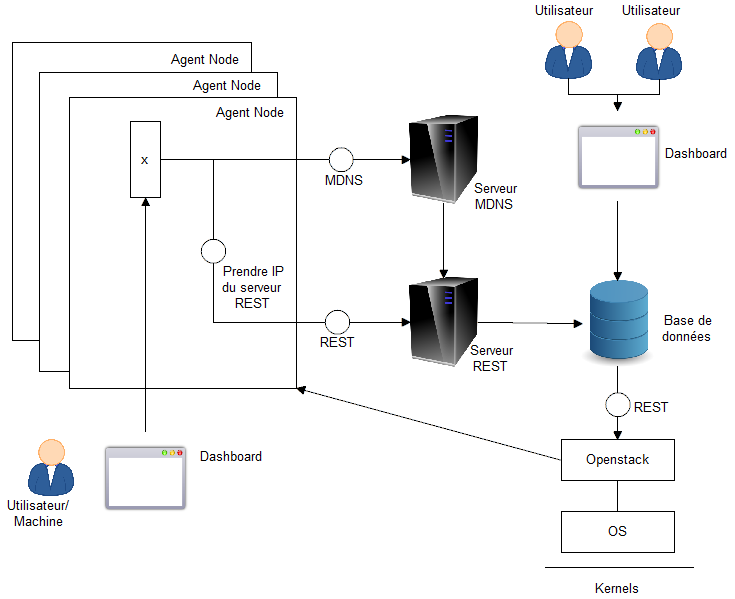
\includegraphics[width=0.7\columnwidth] {../images/schema_architecture.png}
  \end{center}
  \caption{Schéma de l'architecture de l'application  }
  \label{fig:architecture}
\end{figure}

Il y a deux parties distinctes dans cette architecture.

\begin{itemize}
\item La partie Openstack;
\item La partie applicative.
\end{itemize}

\subsubsection{Langage, Python}

L’implémentation est faite avec le langage Python. Dans le cadre de ce projet, Python possède plusieurs avantages : simplicité de syntaxe, rapidité de développement. De plus de nombreuses API sont disponibles ce qui permet de développer la partie applicative plus efficacement dans un laps de temps court.

\subsubsection{Gestion du cloud, Agent OpenStack}

L’agent OpenStack permet une connection à une infrastructure Openstack et une gestion de certains processus de virtualisation afin de pouvoir utiliser la puissance des équipements sur lesquels cet agent est installé, comme un noeud nova-compute standard. Un noeud nova-compute permet d'exécuter des machines virtuelles sur un ordinateur, sous la supervision d’OpenStack. Cet agent est basé sur docker ainsi que sur ubuntu 10.04:
Ce choix est basé sur deux choses :

\begin{itemize}
	\item Docker permet un déploiement rapide et sans dépendance logicielle autre que lui-même
	\item Ubuntu 14.04 est la version imposé par le projet OpenEdgeComputing, car celui-ci ne fonctionne que sur cette distribution linux
\end{itemize}

Le fonctionnement de cet agent est le suivant : 
\begin{itemize}
	\item Il va dans un premier temps récupérer l’adresse ip du serveur OpenStack qui lui correspond via l’agent node
	\item Puis il va s’y connecter pour pouvoir offrir sa puissance de calcul à l’infrastructure OpenStack
\end{itemize}
\subsubsection{Interface utilisateur, Agent Node}

L’interface utilisateur appelé Agent Node permet à un utilisateur de l’application de pouvoir venir mettre des ressources matérielles à disposition. Pour cela une interface listant tous les objets compatibles avec le cloud et OpenStack est à sa disposition. (cf. figure \ref{fig:agent_node})

\begin{figure}[htpb]
  \begin{center}
    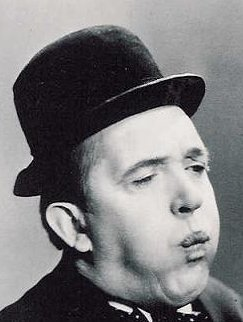
\includegraphics[width=0.7\columnwidth] {../images/SLaurel.jpg}
  \end{center}
  \caption{Image de l'interface utilisateur }
  \label{fig:agent_node}
\end{figure}

En venant cliquer sur le bouton “NOM DU BOUTON”, l’utilisateur enregistre directement son appareil dans la base de donnée où se trouve toutes les ressources mises à disposition  par Orange. Pour cela l’utilisation d’un serveur REST permet un enregistrement simple des différentes ressources et l’utilisation d’un serveur mDNS est nécessaire afin de découvrir les serveurs REST et Openstack. Leurs utilisations sont détaillés dans les sous-parties 4 et 5.

\subsubsection{Processus de découverte, mDNS}

Lorsqu’un utilisateur se connecte à l’interface de l’application, il doit pouvoir mettre à disposition les ressources qu’il souhaite. Pour ce faire, la première étape consiste en la découverte du serveur REST ainsi qu’en la découverte du serveur Openstack. Le protocole mDNS-SD signifie multicast Domain Name Service - Service Discovery. Il s’agit une mécanisme permettant d’adresser des messages dans le réseau sans avoir besoin de savoir avec quel périphérique l’on communique (mDNS). Il permet également de découvrir des services (Service Discovery). Pour mettre en place le service de découverte, la bibliothèque Python, zeroconf a été utilisé . La solution zeroconf permet de découvrir de manière simple les services se situant sur le même réseau. L’implémentation du serveur mDNS permet alors de publier le service du serveur REST, ainsi que du serveur Openstack et ensuite d’en transmettre les informations sur le réseau. Un script permet ensuite à l’Agent Node la découverte de ces serveurs et de communiquer avec.

\subsubsection{Serveur REST}

Une fois la découverte effectué, afin que l’utilisateur puisse mettre à disposition ses appareils, il doit pouvoir enregistrer son appareil dans la base de donnée regroupant toutes les ressources disponibles sur le réseau d’Orange. Pour ce faire, nous avons implémenté un serveur REST (Representational State Transfer). Le serveur REST permet de mettre en à disposition des clients une interface permettant d’envoyer des requêtes via un format défini au préalable et ensuite enregistré les données reçues dans une base de donnée. Nous avons utilisé le format Json, très utilisé et simple d’utilisation.  (cf. figure \ref{fig:json} )

\begin{figure}[htpb]
  \begin{center}
    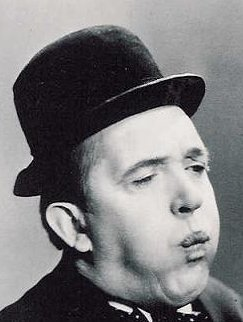
\includegraphics[width=0.7\columnwidth] {../images/SLaurel.jpg}
  \end{center}
  \caption{Exemple de JSon }
  \label{fig:json}
\end{figure}

\subsubsection{Affichage de la base de donnée}

Afin de pouvoir rendre compte du bon enregistrement des appareils dans la base de donnée, nous avons créé une interface affichant la base de donnée. (cf. image dashboard)Afin de pouvoir rendre compte du bon enregistrement des appareils dans la base de donnée, nous avons créé une interface affichant la base de donnée. (cf. figure \ref{fig:dashboard})

\begin{figure}[htpb]
  \begin{center}
    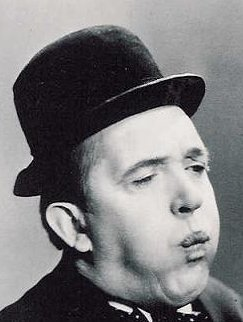
\includegraphics[width=0.7\columnwidth] {../images/SLaurel.jpg}
  \end{center}
  \caption{Représentation de notre Dashboard}
  \label{fig:dashboard}
\end{figure}

\section{Résultats}

\subsection{Recherche sur OpenEdgeComputing}

Les recherches effectués effectués sur OpenEdgeComputing n’ont pas été particulièrement convaincantes. Le projet OpenEdgeComputing est un projet universitaire assez bien documenté, cependant ce projet n’est plus maintenu depuis plus d’un an maintenant (3ans pour le code source). En plus, ce projet OpenEdgeComputing a été partiellement privatisé par les entreprises. Cela explique pourquoi nous avons une diffculté de progresser dans notre recherche. Le deuxième projet traitant de la même problématique est OpenFog cependant ce projet n’en est encore qu'à ses balbutiements, et le premier forum public de ce consortium ne se tiendra qu’en mars. 


\subsection{Mise en place de OpenEdgeComputing}

La mise en place d’OpenEdgeComputing n’a pas été concluante en effet le manque de maintien du projet fait que de nombreux liens notamment au niveau des VMs ne sont plus disponibles. Le projet est à l’heure actuelle très difficilement exploitable et absolument pas prêt pour une quelconque mise en production.

\subsection{Mise en place d'un nouvelle solution}

La nouvelle solution mise en oeuvre est concluante et fonctionne bien d’un point de vue logique à petite échelle : le stack de logiciel fonctionne dans un réseau local sans routeur. Il faudrait cependant déployer cette application à grande échelle afin de voir si celle-ci est scalable.

\section{Analyse}

Une importante partie de notre travail a été consacré à la découverte de Edge Computing et de l’état de l’art des existants. Cependant peu de chose ont été faites dans ce domaine et il nous a fallu repartir de 0 et implémenter notre solution. Celle-ci n’est probablement pas exploitable en l’état à grande échelle mais permet de poser les bases sur lesquelles s’appuyer pour un développement futur plus important.

\section{Discussion}

Le Edge Computing n’en est qu’à ses balbutiements, il n’y a pas encore de standard de disponible sur le marché que cela vienne d’un acteur privé ou du monde de l’open source. Cependant certains paradigmes semble revenir comme le montre l’article (scientifique traité par Merwan a retrovué et a cité). La solution qui a été mise en oeuvre est basé sur ces paradigmes.

\section{Références bibliographiques}

%\\bibliographystyle{IEEEbib} %numérique
%\bibliographystyle{utphys}
%\bibliographystyle{alpha}  %alphanumérique
%\\bibliography{bibliographie}  



\end{document}
